\documentclass{report}
\usepackage[utf8]{inputenc}
\usepackage{listings}
\usepackage{xcolor}
\usepackage{graphicx}
\usepackage{caption} 
\usepackage{helvet}
\usepackage{hyperref}

\renewcommand{\familydefault}{\sfdefault}

\definecolor{codegreen}{rgb}{0,0.6,0}
\definecolor{codegray}{rgb}{0.5,0.5,0.5}
\definecolor{codepurple}{rgb}{0.58,0,0.82}
\definecolor{backcolour}{rgb}{0.95,0.95,0.95}

\lstdefinestyle{mystyle}{
    backgroundcolor=\color{backcolour},   
    commentstyle=\color{codegreen},
    keywordstyle=\color{magenta},
    numberstyle=\tiny\color{codegray},
    stringstyle=\color{codepurple},
    basicstyle=\ttfamily\footnotesize,
    breakatwhitespace=false,         
    breaklines=true,                 
    captionpos=b,                    
    keepspaces=true,                 
    numbers=left,                    
    numbersep=5pt,                  
    showspaces=false,                
    showstringspaces=false,
    showtabs=false,                  
    tabsize=2
}

\lstset{style=mystyle}

\title{PC40 UPC Report}
\author{Esteban Becker}
\date{October 2022}

\begin{document}

\maketitle

\tableofcontents

\chapter{Introduction}

This document is a report of the PC40 UV at the UTBM. \newline
All the tests were run on the \href{https://www.univ-fcomte.fr/informatique-calcul/mesocentre-de-calcul}{mesocentre de calcul Franche-Compté} with 32 execution cores and 64 GB of RAM.\newline
All my code can be found on my GitHub: \href{https://github.com/estebanbecker/Parallel-computing-UPC}{https://github.com/estebanbecker/Parallel-computing-UPC}

\chapter{Work sharing, synchronization}

\section{Conversion table}

To optimize the code, we can parallelize the for loop. To do it correctly, we will not use a test in the loop to distribute the work, but we will change the initiation and the step of the for loop.\newline
We have to add an upc\_barrier to be sure all the work is finished before the results are printed.

\begin{lstlisting}[language=C]
#include <stdio.h>
#include <upc.h>
#define TBL_SZ 12

int main(){
    static shared int fahrenheit[TBL_SZ];
    static shared int step=10; 
    int celsius, i;

    //Create the conversion table
    upc_forall(i=MYTHREAD;i<TBL_SZ;i+=THREADS;i){
        celsius=step*i;
        fahrenheit[i]=celsius*(9.0/5.0)+32;
    }
    //Sync all threads
    upc_barrier;

    //Print the conversion table
    if(MYTHREAD==0)

    for(i=0;i<TBL_SZ;i++){
        celsius=step*i;
        printf("%d \t %d \n", fahrenheit[i], celsius);
    }
}

\end{lstlisting}


\chapter{Shared arrays, blocked shared arrays}



\section{Vector addition}

To add two vectors, we can share the additions between the threads.

\begin{lstlisting}[language=C]
#include<upc_relaxed.h> 
#define N 100 
shared int v1[N], v2[N], v1plusv2[N]; 
void main() 
{ 
    int i; 
    for(i=0;i<N;i++){
        if(MYTHREAD==i%THREADS) 
        v1plusv2[i]=v1[i]+v2[i] ; 
    }
}
\end{lstlisting}

    We can change the loop to avoid the code doing a check at each iteration.

\begin{lstlisting}[language=C]
#include<upc_relaxed.h> 
#define N 100 

shared int v1[N], v2[N], v1plusv2[N]; 
void main() 
{ 
    int i; 
    for(i=MYTHREAD; i<N; i+=THREADS){
        v1plusv2[i]=v1[i]+v2[i] ; 
    }
}
\end{lstlisting}

The shared data are distributed in round rubbish fashion. Here the default distribution yields is an efficient implementation in this case

\section{Matrix vector multiplication}

\begin{lstlisting}[language=C]
shared int a[THREADS][THREADS] ; //Matrix A
shared int b[THREADS], c[THREADS] ; //Vector B and C
void main (void) 

{
    int i, j; 
    //Using upc_forall to share the work
    upc_forall( i = 0 ; i < THREADS ; i++; i){
    c[i] = 0;
        for ( j= 0 ; j < THREADS ; j++){
            c[i] += a[i][j]*b[j];
        }
    }
}
\end{lstlisting}

Here the data is not well distributed because each thread will use data that don't have affinity with it.

\begin{center}
    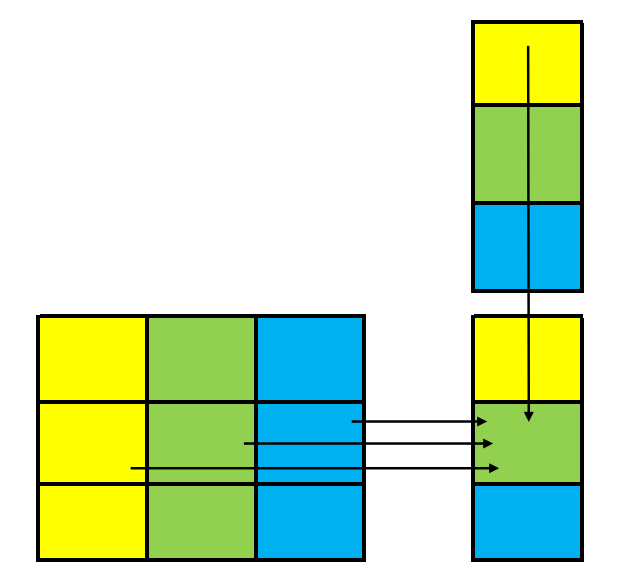
\includegraphics[scale=0.5]{Images/Matrix_vector_unoptimized.png}
    \captionof{figure}{Not optimised data distribution}
    \label{fig1}
\end{center}

To optimize the code, we can change the BLOCKSIZE of the matrix a. With this distribution, all the data of the matrix has affinity to the thread that will use them.

\begin{lstlisting}[language=C]
// vect_mat_mult.c
#include <upc.h>
shared [THREADS] int a[THREADS][THREADS] ; //Matrix A with a different blocksize
shared int b[THREADS], c[THREADS] ; //Vector B and C
void main (void) 

{
    int i, j; 
    //Using upc_forall to share the work
    upc_forall( i = 0 ; i < THREADS ; i++; i){
    c[i] = 0;
        for ( j= 0 ; j < THREADS ; j++){
            c[i] += a[i][j]*b[j];
        }
    }
}
\end{lstlisting}

\begin{center}
    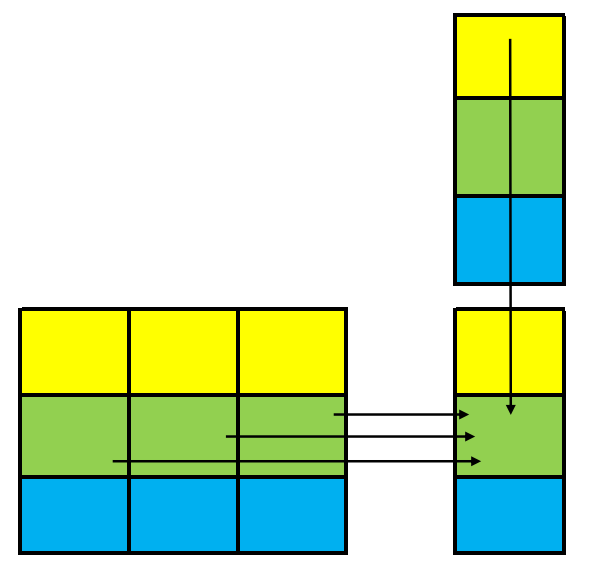
\includegraphics[scale=0.5]{Images/Matrix_vector_optimized.png}
    \captionof{figure}{Optimised data distribution}
    \label{fig2}
\end{center}

\chapter{Simplified 1D Laplace solver}

\section{The 1D solver in UPC}

To implement the 1D Laplace solver in UPC, we can do the following code:

\begin{lstlisting}[language=C]
#include <upc_relaxed.h>
#include <stdio.h>
#include <stdlib.h>
#include <time.h>

#define TOTALSIZE 	800

//== declare the x, x_new, b arrays in the shared space with size of TOTALSIZE
shared double x[TOTALSIZE];
shared double x_new[TOTALSIZE];
shared double b[TOTALSIZE];

void init();

int main(int argc, char **argv){
    int j;

    init();
    upc_barrier;

    //== add a for loop which goes through the elements in the x_new array
    for( j=1; j<TOTALSIZE-1; j++ ){
        //== insert an if statement to do the work sharing across the threads
        if( j % THREADS == MYTHREAD){
            x_new[j] = 0.5*( x[j-1] + x[j+1] + b[j] );
        }
    }

    //Print the result with the first thread
    if( MYTHREAD == 0 ){
        printf("   b   |    x   | x_new\n");
        printf("=============================\n");

        for( j=0; j<TOTALSIZE; j++ )
            printf("%1.4f | %1.4f | %1.4f \n", b[j], x[j], x_new[j]);
    }

    return 0;
}

void init(){
    int i;

    if( MYTHREAD == 0 ){
        srand(time(NULL));

        for( i = 0; i<TOTALSIZE; i++ ){
            b[i] = (double)rand() / RAND_MAX;
            x[i] = (double)rand() / RAND_MAX;
        }
    }
}

\end{lstlisting}

This implementation isn't optimized because each thread will check an IF statement to share the work. 

To avoid the race condition, we can add two upc\_barrier, one after the initialization and another before the printing

\begin{center}
    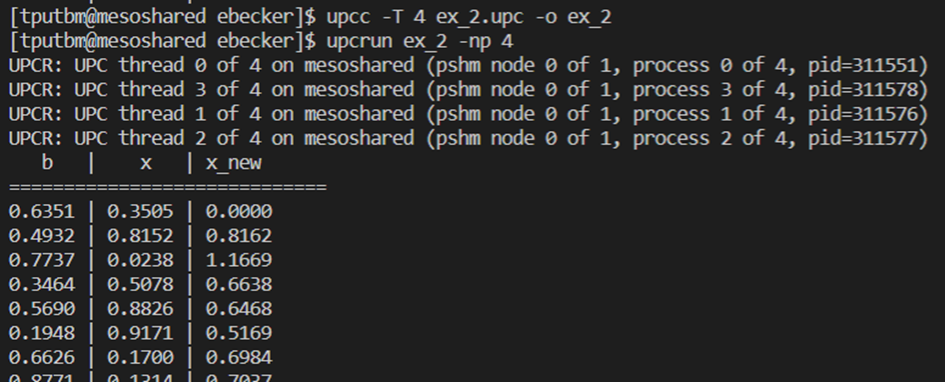
\includegraphics[scale=0.75]{Images/1rst_output.png}
    \captionof{figure}{Output of the 1rst 1D Laplace solver}
    \label{fig3}
\end{center}

\section{Optimize the code}

\subsection{Avoiding the if condition}
To avoid the code to check an if condition, we can use the following for loop:

\begin{lstlisting}[language=C]
    for(int j=MYTHREAD; j<TOTALSIZE-1; j+=THREADS ){
        x_new[j] = 0.5*( x[j-1] + x[j+1] + b[j] );
    }
\end{lstlisting}

\subsection{Blocked arrays}

To optimize the memory distribution, we can set a BLOCKSIZE and change the for loop to an upc\_forall 

\begin{lstlisting}[language=C]
#include <upc_relaxed.h>
#include <stdio.h>
#include <stdlib.h>
#include <time.h>

#define BLOCKSIZE 16

//==> declare the x, x_new and b arrays in the shared space with size of 
//    BLOCKSIZE*THREADS and with blocking size of BLOCKSIZE
shared [BLOCKSIZE] double x[BLOCKSIZE*THREADS];
shared [BLOCKSIZE] double x_new[BLOCKSIZE*THREADS];
shared [BLOCKSIZE] double b[BLOCKSIZE*THREADS];

void init();

int main(int argc, char **argv){
    int j;

    init();
    upc_barrier;
    //==> insert a upc_forall statement to do work sharing while 
    //    respecting the affinity of the x_new array
    upc_forall( j=1; j<(BLOCKSIZE*THREADS)-1; j++; &x_new[j] ){
        x_new[j] = 0.5*( x[j-1] + x[j+1] + b[j] );
    }
    upc_barrier;

    if( MYTHREAD == 0 ){
        printf("   b   |    x   | x_new\n");
        printf("=============================\n");

        for( j=0; j<BLOCKSIZE*THREADS; j++ )
            printf("%1.4f | %1.4f | %1.4f \n", b[j], x[j], x_new[j]);
    }

    return 0;
}

void init(){
    int i;

    if( MYTHREAD == 0 ){
        srand(time(NULL));

        for( i=0; i<BLOCKSIZE*THREADS; i++ ){
            b[i] = (double)rand() / RAND_MAX;
            x[i] = (double)rand() / RAND_MAX;
        }
    }
}


\end{lstlisting}

\begin{center}
    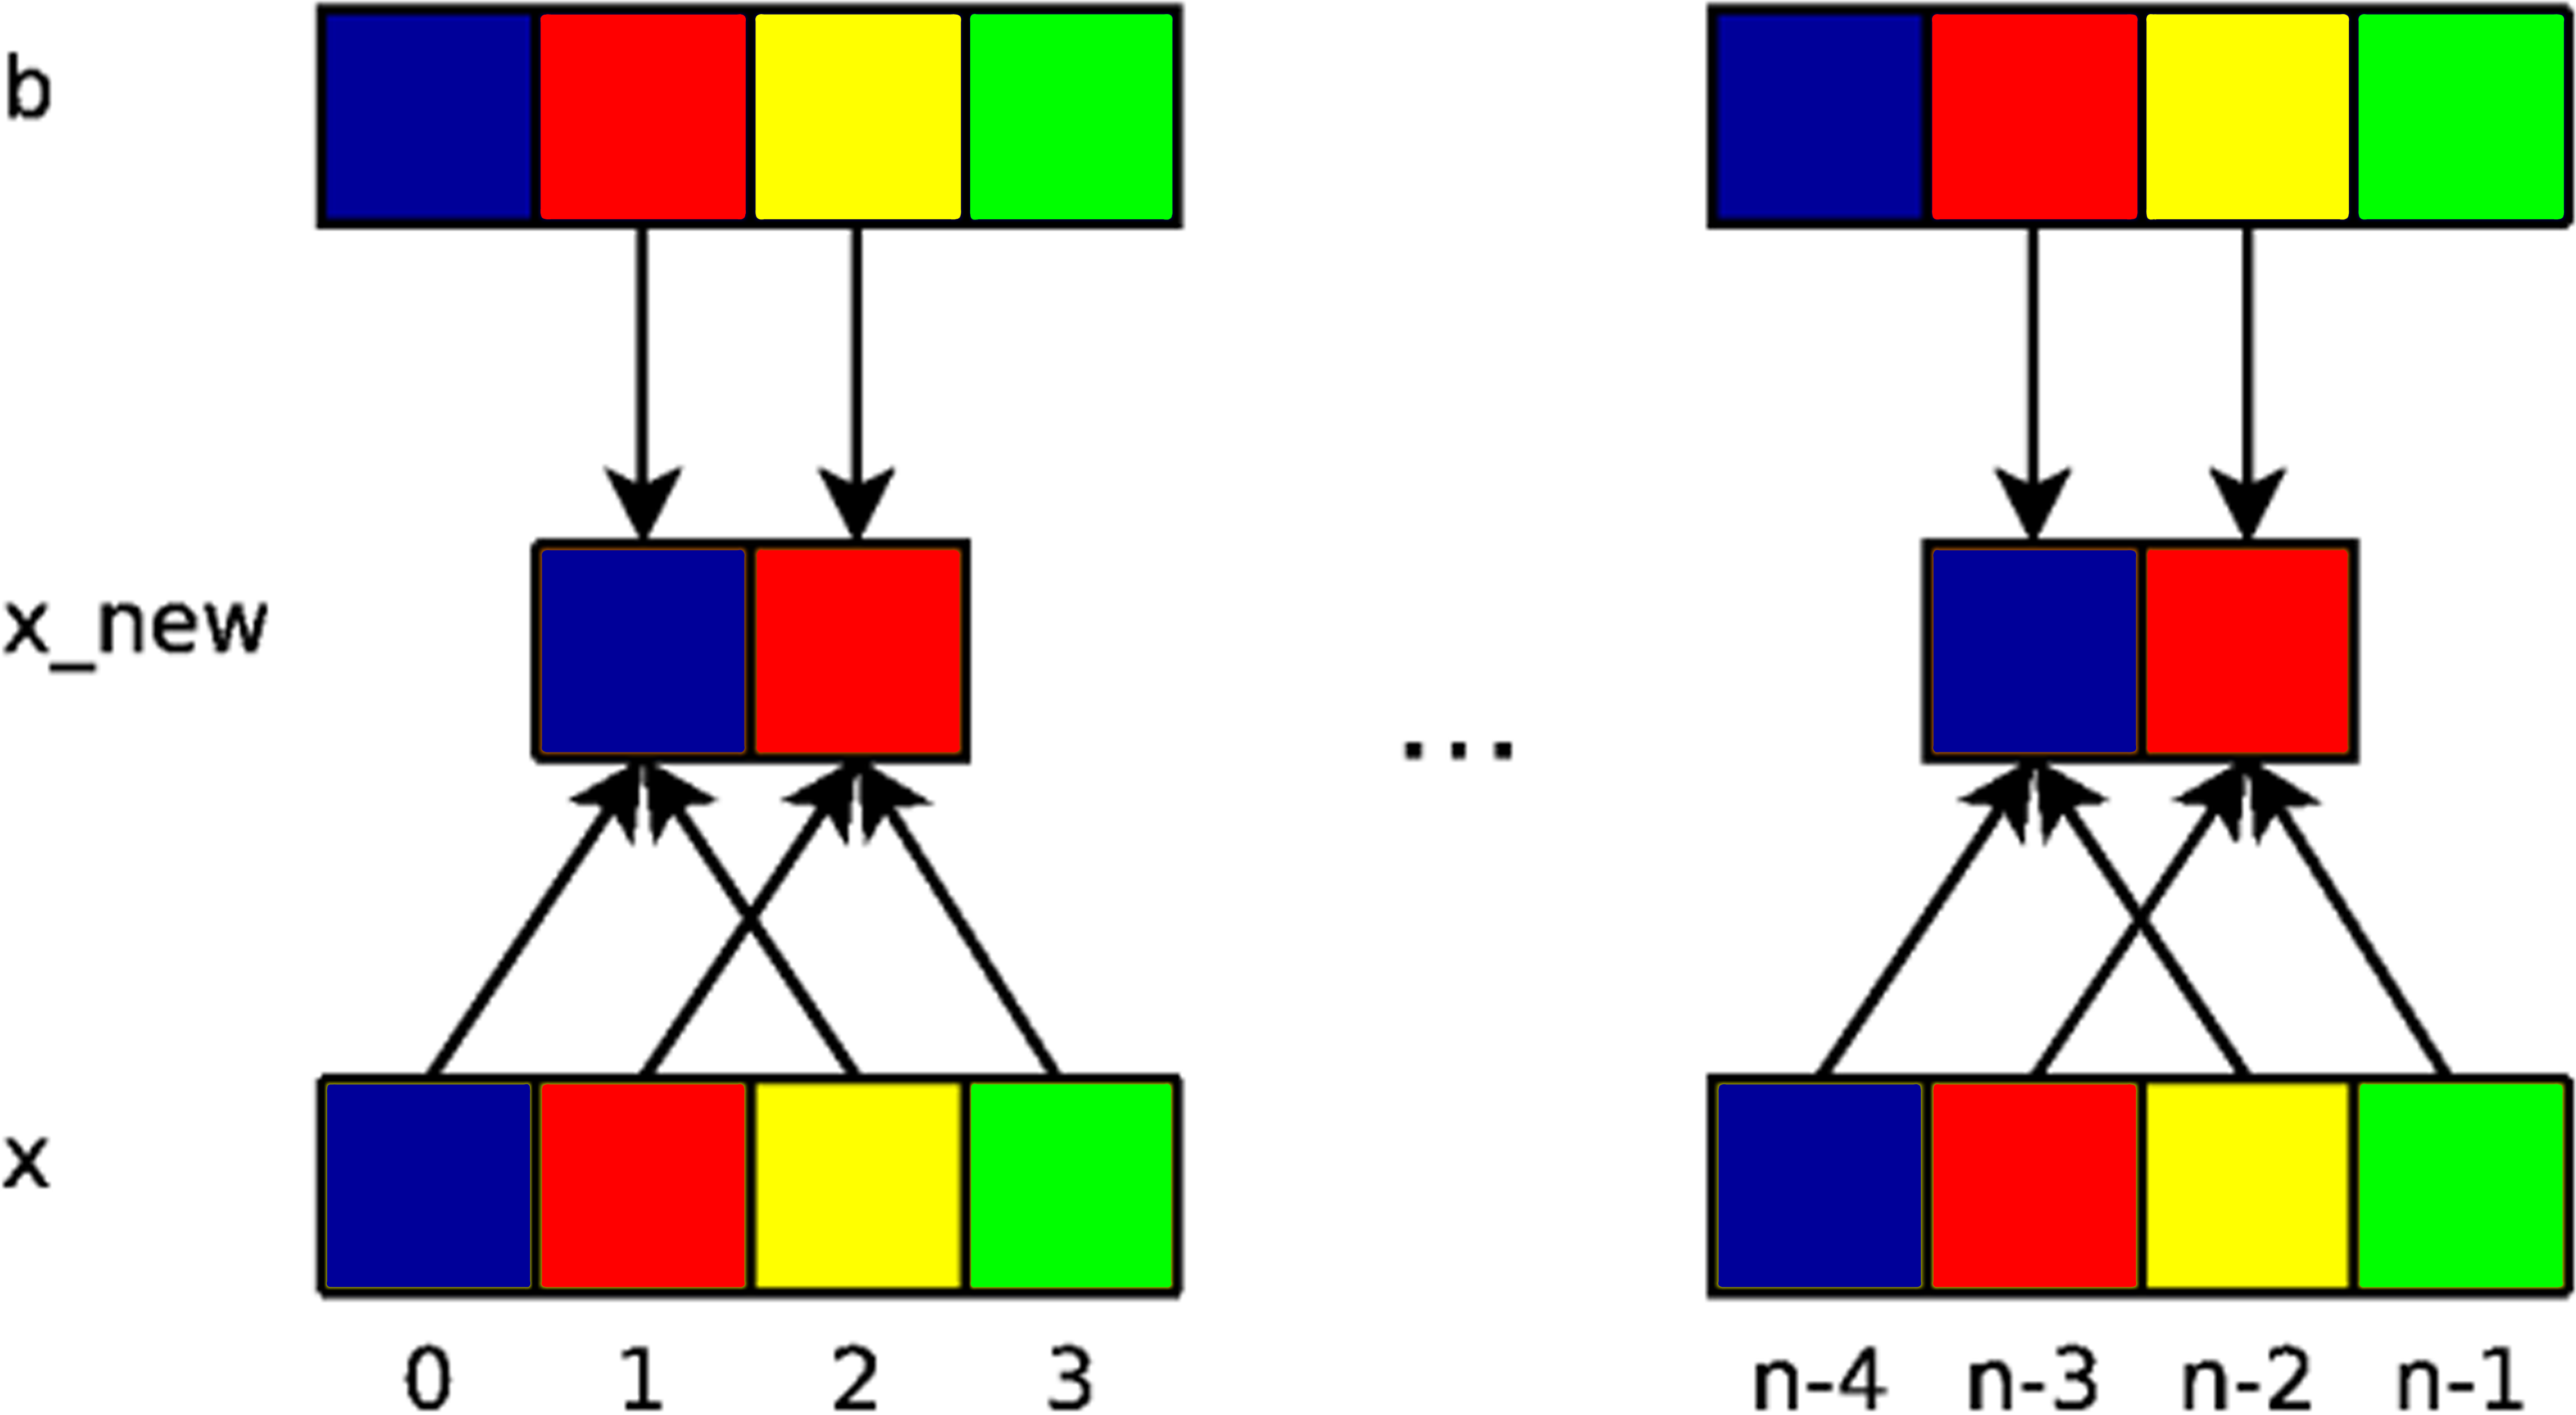
\includegraphics[scale=0.070]{Images/Laplace_unoptimized_da.png}
    \captionof{figure}{Unoptimised data distribution}
    \label{fig4}
    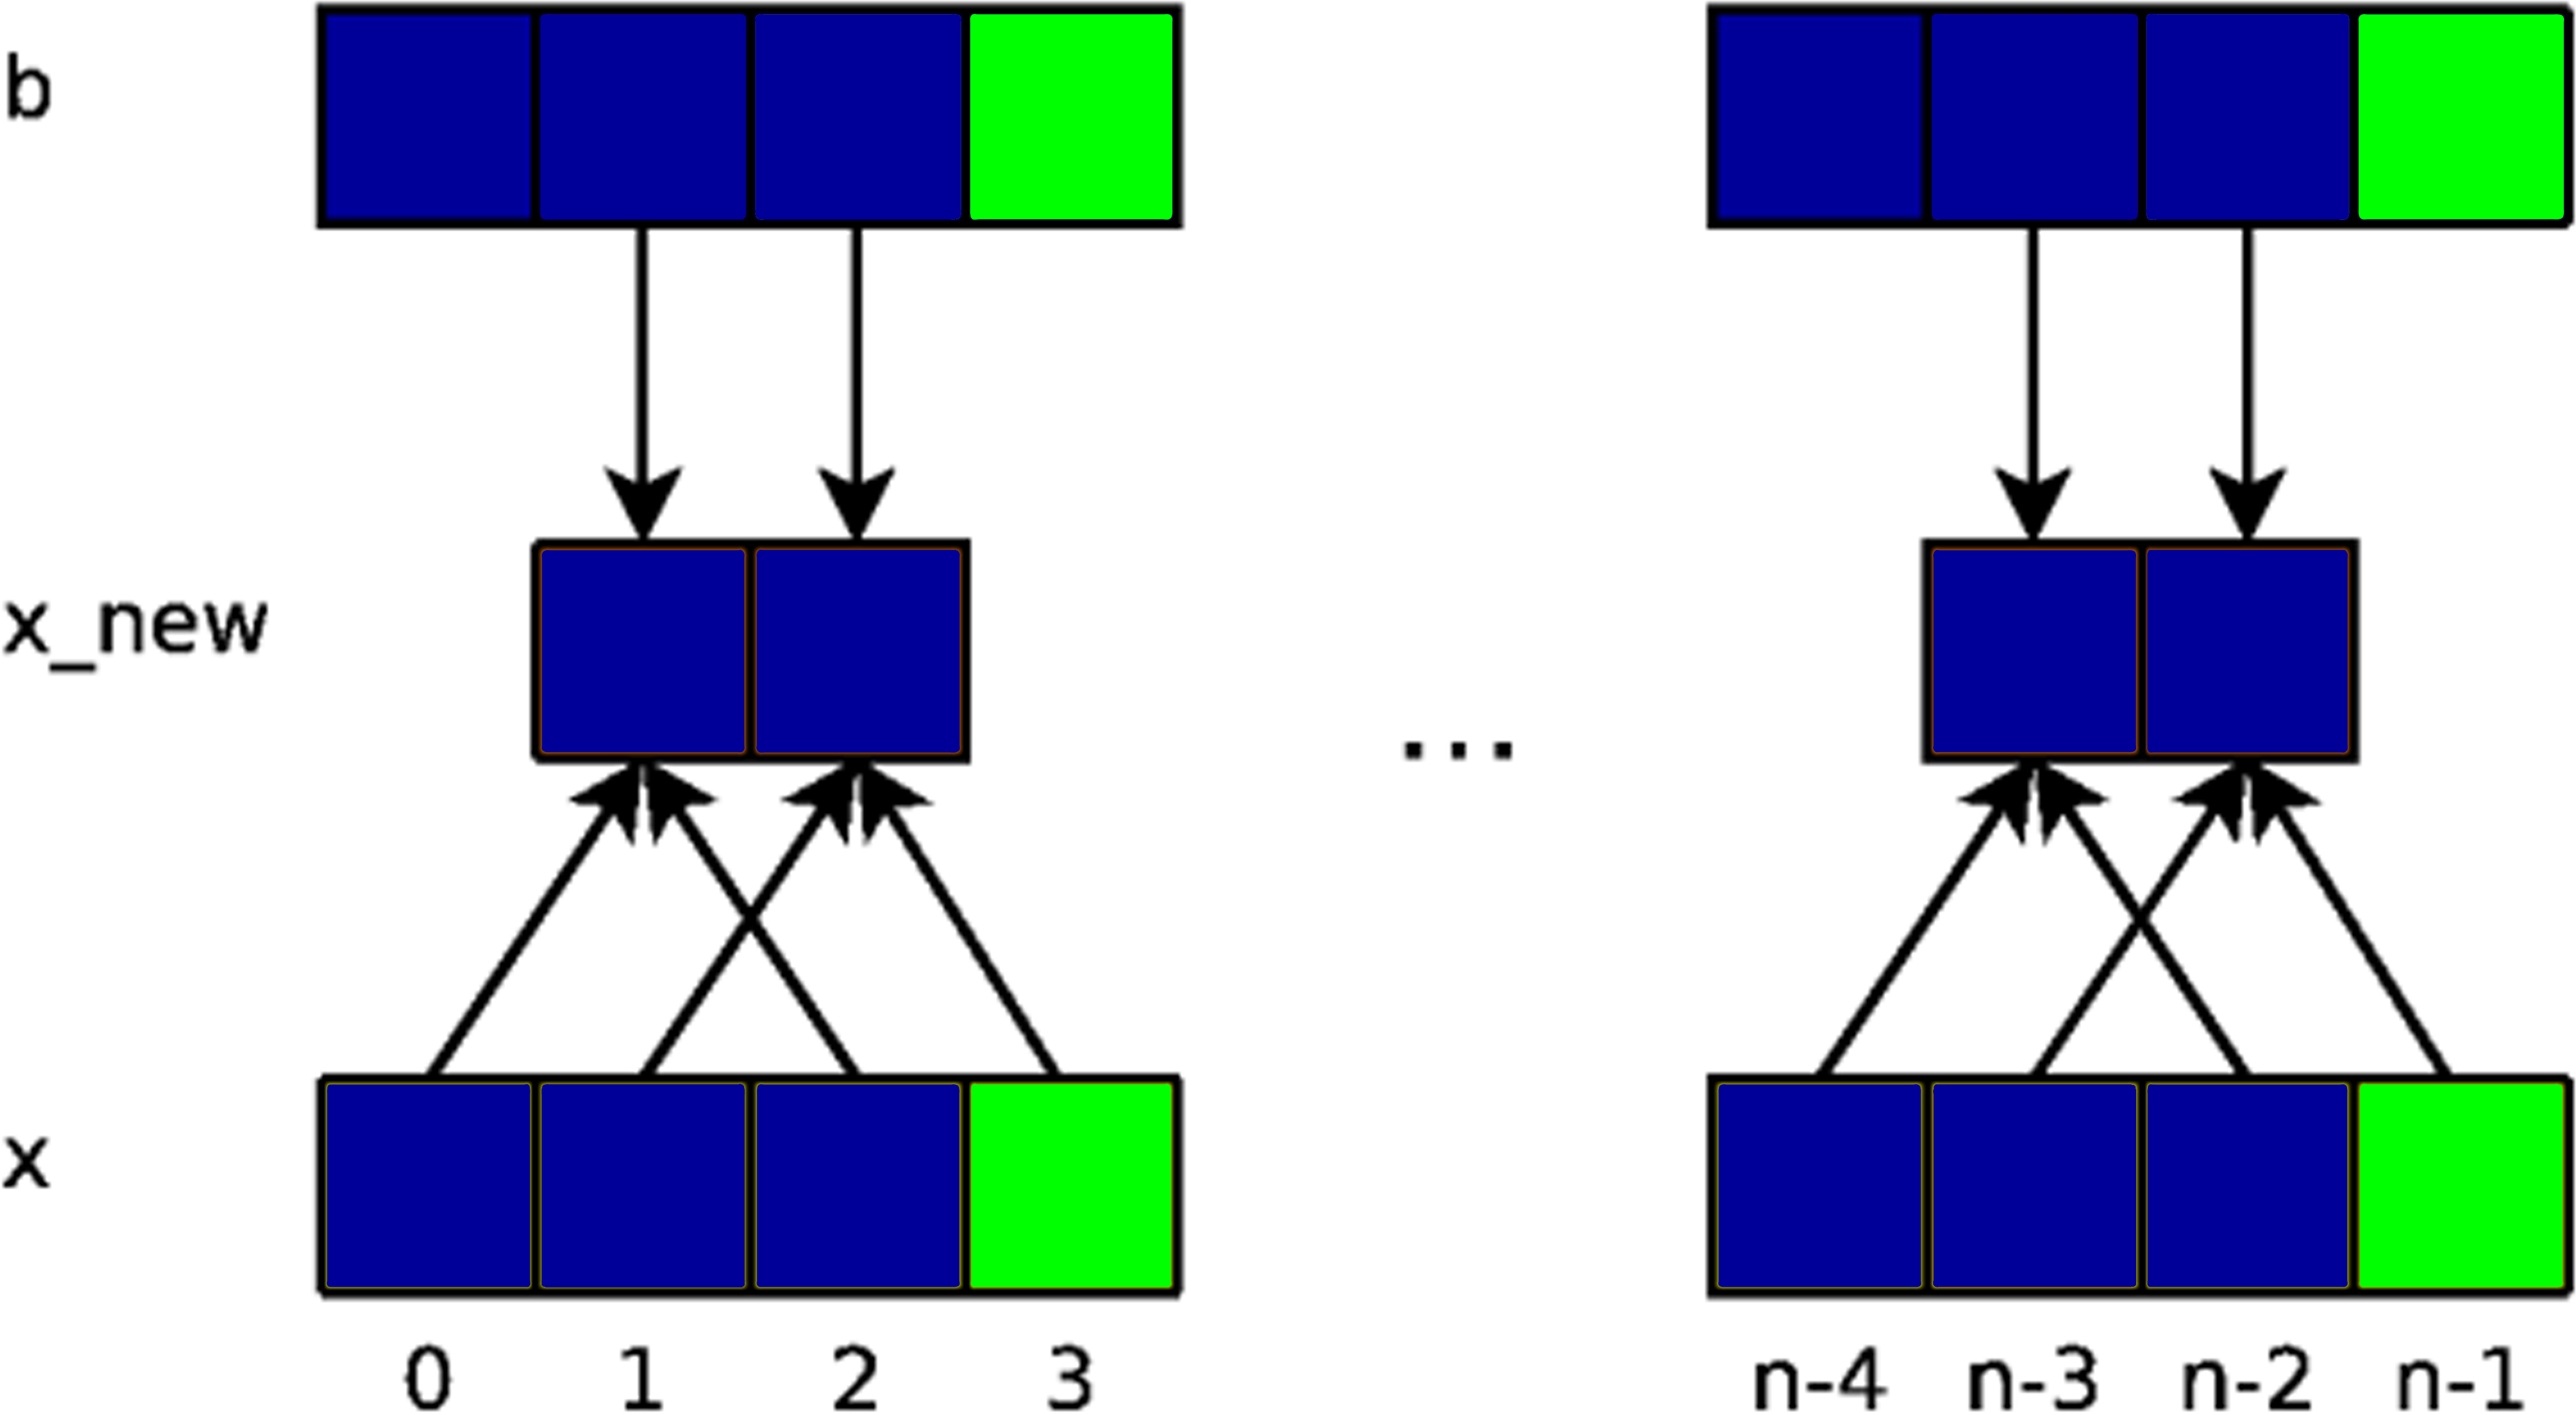
\includegraphics[scale=0.070]{Images/Lapalce_optmized_data.png}
    \captionof{figure}{Optimised data distribution}
    \label{fig5}
\end{center}

With the above schema, we can see that when the data are grouped together, there is more shared memory access with affinity than the original distribution.

\section{Synchronization}

\begin{lstlisting}[language=c]
#include <upc_relaxed.h>
#include <stdio.h>
#include <stdlib.h>
#include <time.h>
#define BLOCKSIZE 16

shared [BLOCKSIZE] double x[BLOCKSIZE*THREADS];
shared [BLOCKSIZE] double x_new[BLOCKSIZE*THREADS];
shared [BLOCKSIZE] double b[BLOCKSIZE*THREADS];

void init();

int main(int argc, char **argv){
    int j;
    int iter;

    init();

    // add two barrier statements, to ensure all threads finished computing
    // x_new[] and to ensure that all threads have completed the array
    // swapping.
    for( iter=0; iter<10000; iter++ ){
        upc_forall( j=1; j<BLOCKSIZE*THREADS-1; j++; &x_new[j] ){
            x_new[j] = 0.5*( x[j-1] + x[j+1] + b[j] );
        }

        //UPC barrier needed to ensure all threads have finished computing x_new[]
        upc_barrier;

        upc_forall( j=0; j<BLOCKSIZE*THREADS; j++; &x_new[j] ){
            x[j] = x_new[j];
        }

        //UPC barrier needed to ensure all threads have finished swapping x[] and x_new[]
        upc_barrier;
    }

    if( MYTHREAD == 0 ){
        printf("   b   |    x   | x_new\n");
        printf("=============================\n");

        for( j=0; j<BLOCKSIZE*THREADS; j++ )
            printf("%1.4f | %1.4f | %1.4f \n", b[j], x[j], x_new[j]);
    }

    return 0;
}

void init(){
    int i;

    if( MYTHREAD == 0 ){
        srand(time(NULL));

        for( i=0; i<BLOCKSIZE*THREADS; i++ ){
            b[i] = (double)rand() / RAND_MAX;
            x[i] = (double)rand() / RAND_MAX;
        }
    }
    upc_barrier;
}

\end{lstlisting}

To implement the iteration, we have to avoid the race condition by adding two upc\_barrier at the lines 28 and 35

\section{Convergence}
We have to keep track of the maximum difference between the \textit{x} and \textit{xmax}.
To check if the code reached to convergence, we can use the following collective operation:
\begin{lstlisting}[language=c]
upc_all_reduceD( &diffmax, diff, UPC_MAX,THREADS,1,NULL,UPC_OUT_ALLSYNC);
\end{lstlisting}

Finally, we obtain this code:

\begin{lstlisting}[language=c]
#include <upc.h>
#include <upc_collective.h> 
#include <stdio.h>
#include <math.h>

#define TOTALSIZE 100
#define EPSILON 0.000001

shared [TOTALSIZE] double x[TOTALSIZE*THREADS];
shared [TOTALSIZE] double x_new[TOTALSIZE*THREADS];
shared [TOTALSIZE] double b[TOTALSIZE*THREADS];
shared double diff[THREADS];
shared double diffmax;

void init(){
    int i;

    for( i = 0; i < TOTALSIZE*THREADS; i++ ){
        b[i] = 0;
        x[i] = 0;
    }

    b[1] = 1.0;
    b[TOTALSIZE*THREADS-2] = 1.0;
}

int main(){
    int j;
    int iter = 0;

    if( MYTHREAD == 0 )
        init();

    upc_barrier;

    while( 1 ){
        iter++;
        diff[MYTHREAD] = 0.0;

        upc_forall( j=1; j<TOTALSIZE*THREADS-1; j++; &x_new[j] ){
            x_new[j] = 0.5 * ( x[j-1] + x[j+1] + b[j] );

            if( diff[MYTHREAD] < x_new[j] - x[j] )
                diff[MYTHREAD] = x_new[j] - x[j];
        }

        // Each thread as a local value for diff
        // The maximum of those values should be used to check
        // the convergence.

        upc_all_reduceD( &diffmax, diff, UPC_MAX,THREADS,1,NULL,UPC_OUT_ALLSYNC);

        printf("diff max = %f \n", diffmax);

        if( diffmax <= EPSILON )
            break;
        if( iter > 10000 )
            break;

        upc_forall( j=0; j<TOTALSIZE*THREADS; j++; &x_new[j] ){
            x[j] = x_new[j];
        }
        upc_barrier;
    }

    
    if( MYTHREAD == 0 ){
        for(j=0; j<TOTALSIZE*THREADS; j++){
            printf("%f\t", x_new[j]);
        }
        printf("\n");
    }

    return 0;
}
\end{lstlisting}

\chapter{2D Heat conduction}

\section{First UPC program}

To create the first UPC version, we spread the work between all the threads and optimize the data blocksize.

\begin{lstlisting}[language=c]
#include <stdio.h>
#include <math.h>
#include <sys/time.h>
#include <upc_relaxed.h>
#include <upc_collective.h> 

#define N 30

shared [(N+2)*(N+2)/THREADS] double grid[N+2][N+2], new_grid[N+2][N+2];
shared double dTmax[THREADS];
shared double diffmax;

void initialize(void)
{
    int j;

    /* Heat one side of the solid */
    upc_forall( j=1; j<N+1; j++; j)
    {
        grid[0][j] = 1.0;
        new_grid[0][j] = 1.0;
    }
    upc_barrier;
}

int main(void)
{
    struct timeval ts_st, ts_end;
    double dT, epsilon, time;
    int finished, i, j, k, l;
    double T;
    int nr_iter;

    initialize();

    /* Set the precision wanted */
    epsilon  = 0.0001;
    finished = 0;
    nr_iter = 0;

    /* and start the timed section */
    gettimeofday( &ts_st, NULL );

    do
    {
        dTmax[MYTHREAD] = 0.0; 
        upc_forall( i=1; i<N+1; i++; i*THREADS/(N+2))
        {
            //Do the new grid calculation
            for( j=1; j<N+1; j++ )
            {
                T = 0.25 *
                    (grid[i+1][j] + grid[i-1][j] +
                     grid[i][j-1] + grid[i][j+1]); /* stencil */
                dT = T - grid[i][j]; /* local variation */
                new_grid[i][j] = T;
                if( dTmax[MYTHREAD] < fabs(dT) )
                    dTmax[MYTHREAD] = fabs(dT); /* max variation in this iteration */
            }
        }
        upc_barrier;
        upc_all_reduceD( &diffmax, dTmax, UPC_MAX,THREADS,1,NULL,UPC_OUT_ALLSYNC);
        if( diffmax < epsilon ) /* is the precision reached good enough ? */
            finished = 1;
        else
        {
            upc_forall( k=0; k<N+2; k++; k)      /* swap the grids */
                for( l=0; l<N+2; l++ )    
                    grid[k][l] = new_grid[k][l]; 
        }
        upc_barrier;
        nr_iter++;
    } while( finished == 0 );

    if(MYTHREAD == 0)
    {
        gettimeofday( &ts_end, NULL ); /* end the timed section */

        /* compute the execution time */
        time = ts_end.tv_sec + (ts_end.tv_usec / 1000000.0);
        time -= ts_st.tv_sec + (ts_st.tv_usec / 1000000.0);

        printf("%d iterations in %.3lf sec\n", nr_iter, time);
    }

    return 0;
}
\end{lstlisting}

\section{Better memory use}

We can improve the memory use by not copying the whole grid at each iteration. To do that, we will use a pointer for each grid and flip them at the end of an iteration.\newline
To achieve that, we have to declare shared pointers:
\begin{lstlisting}[language=c]
shared [(N+2)*(N+2)/THREADS] double *shared ptr[N+2], *shared new_ptr[N+2];
\end{lstlisting}
And change the copying part of the code with a pointer flipping step:

\begin{lstlisting}[language=c]
upc_forall( k=0; k<N+2; k++; k)
    {   
        tmp = ptr[k];
        ptr[k] = new_ptr[k];
        new_ptr[k] = tmp;
    }
\end{lstlisting}

\section{Performance boost using privatization}

To increase the performance, we can use private pointers. To do that, we will have to do 3 different for loop. One for the top part of the local pointers, one for the middle part and one for the bottom part.

\begin{center}
    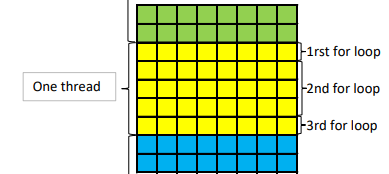
\includegraphics[scale=1]{Images/for_loop_distribution.png}
    \captionof{figure}{The 3 different for loop}
    \label{fig6}
\end{center}

\begin{lstlisting}[language=c]
#include <stdio.h>
#include <math.h>
#include <sys/time.h>
#include <upc_relaxed.h>
#include <upc_collective.h> 

#define N 30
#define PRIV_SIZE ((N+2)/THREADS)

shared [(N+2)*(N+2)/THREADS] double grid[N+2][N+2], new_grid[N+2][N+2];
shared double dTmax[THREADS];
shared double diffmax;
double *new_ptr_priv[PRIV_SIZE], *ptr_priv[PRIV_SIZE], *tmp_priv;
shared [(N+2)*(N+2)/THREADS] double *ptr[N+2], *new_ptr[N+2], *tmp;

void initialize(void)
{
    int j;

    /* Heat one side of the solid */
    for(j=1;j<N+1; j++)
    {
        grid[0][j] = 1.0;
        new_grid[0][j] = 1.0;
    }
}

int main(void)
{
    struct timeval ts_st, ts_end;
    double dT, epsilon, time;
    int finished, i, j, k, l;
    double T;
    int nr_iter;

    if(MYTHREAD == 0)
    {
        initialize();
    }
    upc_barrier;
    /* Set the precision wanted */
    epsilon  = 0.0001;
    finished = 0;
    nr_iter = 0;

    /*Initialize the pointers*/
    for (i = 0; i < N + 2; i++)
    {
        ptr[i] = grid[i];
        new_ptr[i] = new_grid[i];
    }

    for (i = 0; i < PRIV_SIZE; i++)
    {
        ptr_priv[i] = (double *) grid[i + (MYTHREAD * PRIV_SIZE)];
        new_ptr_priv[i] = (double *) new_grid[i + (MYTHREAD * PRIV_SIZE)];
    }   

    /* and start the timed section */
    gettimeofday( &ts_st, NULL );

    do
    {
        dTmax[MYTHREAD] = 0.0;
        if(MYTHREAD!=0)
        {
            /*First for loop for the first line*/
            for( j=1; j<N+1; j++ )
            {  
                i=0;
                T = 0.25 *
                    (ptr_priv[i + 1][j] + ptr[(MYTHREAD*PRIV_SIZE)-1][j] +
                     ptr_priv[i][j-1] + ptr_priv[i][j+1]); /* stencil */
                
                dT = T - ptr_priv[0][j]; /* local variation */
                if( fabs(dT) > dTmax[MYTHREAD] )
                    dTmax[MYTHREAD] = fabs(dT);
                new_ptr_priv[i][j] = T;
            }
        }
        
        /*Second for loop for the lines in the middle with only private pointers*/
        for( i=1; i<(N+2)/THREADS-1; i++)
        {
            for( j=1; j<N+1; j++ )
            {
                T = 0.25 *
                    (ptr_priv[i+1][j] + ptr_priv[i-1][j] +
                     ptr_priv[i][j-1] + ptr_priv[i][j+1]); /* stencil */
                dT = T - ptr_priv[i][j]; /* local variation */
                
                if( fabs(dT) > dTmax[MYTHREAD] )
                    dTmax[MYTHREAD] = fabs(dT);
    
                new_ptr_priv[i][j] = T;
            }
        }

        /*Third for loop for the last line*/
        if(MYTHREAD!=THREADS-1)
        {
            for( j=1; j<N+1; j++ )
            {
                T = 0.25 *
                    (ptr[(MYTHREAD + 1)* PRIV_SIZE][j] + ptr_priv[i-1][j] +
                     ptr_priv[i][j-1] + ptr_priv[i][j+1]); /* stencil */
                dT = T - ptr_priv[i][j]; /* local variation */

                if( fabs(dT) > dTmax[MYTHREAD] )
                    dTmax[MYTHREAD] = fabs(dT);
                new_ptr_priv[i][j] = T;
            }
        }
        upc_all_reduceD( &diffmax, dTmax, UPC_MAX,THREADS,1,NULL,UPC_IN_ALLSYNC | UPC_OUT_ALLSYNC);

        
        if( diffmax < epsilon ) /* is the precision reached good enough ? */
            finished = 1;
        else
        {
            /*Swap the pointers*/
            upc_forall(k = 0 ; k<N+2 ; k++ ; k)   
            {   
                tmp = ptr[k];
                ptr[k] = new_ptr[k];
                new_ptr[k] = tmp;  
            }
            for( l=0; l<PRIV_SIZE; l++)
            {
                tmp_priv = ptr_priv[l];
                ptr_priv[l] = new_ptr_priv[l];
                new_ptr_priv[l] = tmp_priv;
            }
        }
        upc_barrier;
        nr_iter++;
    } while( finished == 0 );

    if(MYTHREAD == 0)
    {
        gettimeofday( &ts_end, NULL ); /* end the timed section */

        /* compute the execution time */
        time = ts_end.tv_sec + (ts_end.tv_usec / 1000000.0);
        time -= ts_st.tv_sec + (ts_st.tv_usec / 1000000.0);

        printf("%d iterations in %.5lf sec\n", nr_iter, time);
    }
    
    return 0;
}
\end{lstlisting}

\section{Dynamic problem size}

To allow the user to choose the problem size at the run time in the command, we will have to use memory allocation with upc\_alloc and malloc.

\begin{lstlisting}[language=c]
#include <stdio.h>
#include <math.h>
#include <sys/time.h>
#include <upc_relaxed.h>
#include <upc_collective.h> 

#define grid(i,j) sh_grid[(((i) * (N+2)) + (j))/((N+2)*priv_size)].chunk[(((i) * (N+2)) + (j))%((N+2)*priv_size)]
#define new_grid(i,j) sh_new_grid[(((i) * (N+2)) + (j))/((N+2)*priv_size)].chunk[(((i) * (N+2)) + (j))%((N+2)*priv_size)]

#define priv_grid(i,j) *ptr_priv[(((i) * (N+2)) + (j))]
#define priv_new_grid(i,j) *new_ptr_priv[(((i) * (N+2)) + (j))]

shared double dTmax[THREADS];
shared double diffmax;
int N;
int priv_size;

typedef struct chunk_s chunk_t;
struct chunk_s {
    shared [] double *chunk;
};

shared chunk_t sh_grid[THREADS];
shared chunk_t sh_new_grid[THREADS];
chunk_t tmp;

void initialize(void)
{
    int j;

    /* Heat one side of the solid */
    for(j=1;j<N+1; j++)
    {
        grid(0,j) = 1.0;
        new_grid(0,j) = 1.0;
    }
}

int main(int argc, char *argv[])
{
    struct timeval ts_st, ts_end;
    double dT, epsilon, time;
    int finished, i, j, k, l;
    double T;
    int nr_iter;


    if(argc != 2)
    {
        if(MYTHREAD == 0)
        {
            printf("Usage: %s <N>", argv[0]);
        }        
        exit(1);
    }
    N = atoi(argv[1]);
    if(N<1)
    {
        if(MYTHREAD == 0)
        {
            printf("N must be greater than 1");
        }
        exit(1);
    }
    priv_size = (N+2)/THREADS;

    /*Alocate the memory*/
    sh_grid[MYTHREAD].chunk = (shared[] double *) upc_alloc((N+2)*priv_size*sizeof(double));
    sh_new_grid[MYTHREAD].chunk = (shared[] double *) upc_alloc((N+2)*priv_size*sizeof(double));

    if(MYTHREAD == 0)
    {
        initialize();
    }
    /* Set the precision wanted */
    epsilon  = 0.0001;
    finished = 0;
    nr_iter = 0;

    /*Alloc the private pointers*/
    double **ptr_priv = (double **) malloc((N+2)*priv_size*sizeof(double*));
    double **new_ptr_priv = (double **) malloc((N+2)*priv_size*sizeof(double*));


    /*Initialize the pointers*/
    for (i = 0; i < (N+2)*priv_size; i++)
    {
        ptr_priv[i] = (double *) &sh_grid[MYTHREAD].chunk[i];
        new_ptr_priv[i] = (double *) &sh_new_grid[MYTHREAD].chunk[i];
    }

    upc_barrier;
    /* and start the timed section */
    gettimeofday( &ts_st, NULL );

    do
    {
        dTmax[MYTHREAD] = 0.0;
        if(MYTHREAD!=0)
        {
            /*First for loop for the first line*/
            for( j=1; j<N+1; j++ )
            {  
                i=0;
                T = 0.25 *
                    (priv_grid(i + 1,j) + grid((MYTHREAD*priv_size)-1,j) +
                     priv_grid(i,j-1) + priv_grid(i,j+1)); /* stencil */

                dT = T - priv_grid(i,j); /* local variation */
                if( fabs(dT) > dTmax[MYTHREAD] )
                    dTmax[MYTHREAD] = fabs(dT);
                priv_new_grid(i,j) = T;
            }
        }
        
        /*Second for loop for the lines in the middle with only private pointers*/
        for( i=1; i<(N+2)/THREADS-1; i++)
        {
            for( j=1; j<N+1; j++ )
            {  
                T = 0.25 *
                    (priv_grid(i + 1,j) + priv_grid(i - 1,j) +
                     priv_grid(i,j-1) + priv_grid(i,j+1)); /* stencil */
                
                dT = T - priv_grid(i,j); /* local variation */

                if( fabs(dT) > dTmax[MYTHREAD] )
                    dTmax[MYTHREAD] = fabs(dT);
                priv_new_grid(i,j) = T;
            }
        }

        if(MYTHREAD!=THREADS-1)
        {
            /*Third for loop for the last line*/
            for( j=1; j<N+1; j++ )
            {  
                i=(N+2)/THREADS-1;
                T = 0.25 *
                    (priv_grid(i,j + 1) + priv_grid(i - 1,j) +
                     priv_grid(i,j-1) + grid((MYTHREAD+1)*priv_size,j)); /* stencil */

                dT = T - priv_grid(i,j); /* local variation */
                if( fabs(dT) > dTmax[MYTHREAD] )
                    dTmax[MYTHREAD] = fabs(dT);
                priv_new_grid(i,j) = T;
            }
        }

        upc_barrier;

        diffmax = 0.0;

        /*Calcul the diffmax for all the threads*/
        for(i=0; i<THREADS; i++)
        {
            if(dTmax[i] > diffmax)
            {
                diffmax = dTmax[i];
            }
        }

        upc_all_reduceD( &diffmax, dTmax, UPC_MAX,THREADS,1,NULL,UPC_IN_ALLSYNC | UPC_OUT_ALLSYNC);

        if( diffmax < epsilon ) /* is the precision reached good enough ? */
            finished = 1;
        else
        {
            /*switch the matrix*/
            shared double *tmp;
            tmp = sh_grid[MYTHREAD].chunk;
            sh_grid[MYTHREAD].chunk = sh_new_grid[MYTHREAD].chunk;
            sh_new_grid[MYTHREAD].chunk = tmp;


            double ** tmp_priv;
            tmp_priv = ptr_priv;
            ptr_priv = new_ptr_priv;
            new_ptr_priv = tmp_priv;
        }
        upc_barrier;
        nr_iter++;
    } while( finished == 0 );

    if(MYTHREAD == 0)
    {
        gettimeofday( &ts_end, NULL ); /* end the timed section */

        /* compute the execution time */
        time = ts_end.tv_sec + (ts_end.tv_usec / 1000000.0);
        time -= ts_st.tv_sec + (ts_st.tv_usec / 1000000.0);

        printf("%d iterations in %.5lf sec\n", nr_iter, time);
    }
    /*Free the allocated memory*/
    free(ptr_priv);
    free(new_ptr_priv);

    upc_free(sh_grid[MYTHREAD].chunk);
    upc_free(sh_new_grid[MYTHREAD].chunk);
    return 0;
}
\end{lstlisting}

The grid is defined with chunks in a structure, because we can't define the blocksize at the compilation. But with this code, we can't access the table in a normal way. The line 7 to 11 are here to allow us to use easily the grid in the program.

\section{Analysing the results}

All the tests of this part has been run 10 times to get an average value

\subsection{Comparing the effect of N}

To study the effect of N we will use 16 threads. N is the size of the grid.

\begin{center}
    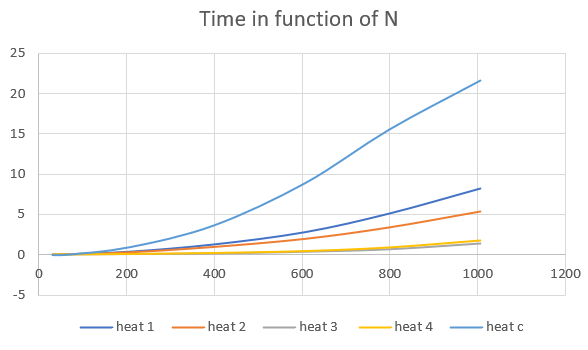
\includegraphics[scale=1]{Images/time_function_of_N.png}
    \captionof{figure}{Graphics of the time in function of N}
    \label{fig7}
\end{center}

On this graph, we can see that when N is bigger, all the run times increase. The C version is the slowest version.

\begin{center}
    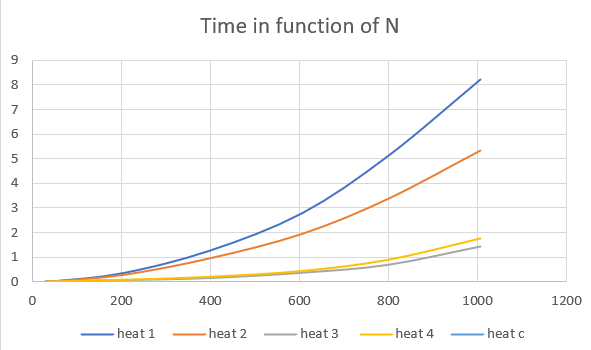
\includegraphics[scale=1]{Images/time_function_N_no_C.png}
    \captionof{figure}{Graphics of the time in function of N without the C version}
    \label{fig8}
\end{center}

There is a big difference between the run time of heat 1, heat 2 and heat 3. With this graph, we can visualize the need to optimize the data distribution and using as much as possible privates pointers and data with affinity.

\subsection{Comparing the speed-up in function of N}

\begin{center}
    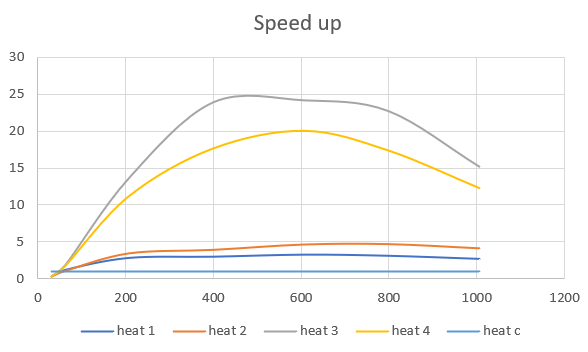
\includegraphics[scale=1]{Images/speed-up_function_N.png}
    \captionof{figure}{Graphics of the speed-up on in function of N}
    \label{fig9}
\end{center}

On this graph we can see that, even if the speed-up is bigger than one for heat 1 and heat 2, having a program (heat 3 and 4) with local data helps a lot.
We can also observe that for small grids, the parallelized version is slower than the c version. 

\begin{table}[h]
\centering
\caption{Speed-up of heat 4 on heat 3}
\label{tab:my-table}
\begin{tabular}{l|l}
N    & Speed-up of heat 4 in function of heat 3 \\ \hline
30   & 0.88                                     \\
62   & 0.92                                     \\
206  & 0.81                                     \\
398  & 0.73                                     \\
606  & 0.82                                     \\
798  & 0.76                                     \\
1006 & 0.80                                    
\end{tabular}
\end{table}

But the most advanced version of heat is slower than heat 3. This can be explained because in heat 4 we have to do a calculation to access the data in the heat table that will slow the program. The flexibility of the program is at the cost of performance, but it's still faster than all the others versions.

\subsection{Comparing the effect of the number of threads}

To compare the effect of the number of threads, N is defined as, 1006

\begin{center}
    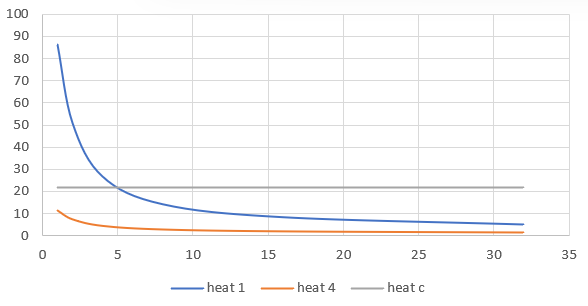
\includegraphics[scale=1]{Images/Time_depending_threads.png}
    \captionof{figure}{Graphics of the time in function of number of threads}
    \label{fig10}
\end{center}

We can see that when the number of threads is bigger, the program is faster. Heat 1 is slower than heat c for 1 threads probably cause all the grid are in shared space, so each pointer to the data must be converted at each call and with one threads there isn't any parallelization. On the other hand, heat 4 is faster because it uses a pointer flipping to exchange the grid instead of the c version that copy the whole grid.

\subsection{Comparing the speed-up in function of the number of threads}

\begin{center}
    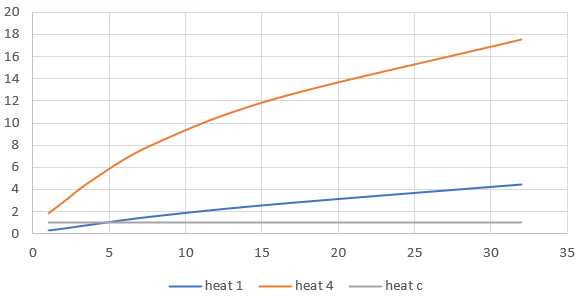
\includegraphics[scale=1]{Images/speeed_up_depending_threads.png}
    \captionof{figure}{Graphics of the speed-up in function of number of threads}
    \label{fig11}
\end{center}

We can observe that when the number of threads is higher, the speed-up of the parallelized version is higher. But the speed-up of the optimized version is way bigger than the not optimized version.

\subsection{Sum up of the results}

We observed that the parallelized version are faster when we have a lot of threads available and a lot of data to work on. It's important when we are running our test to work with a lot of data cause with small N the C version was faster. 

We also observed that one important thing is to optimize the data distribution to use as much local variable and shared data with affinity as possible. There is an average speed-up of 4,8 between heat 4 and heat 1.

We have also seen that the flexibility of a program is at the cost of the performance of this program.

\listoffigures
\end{document}
